\scanpage{108}
% archive foliation: 107
% Pale reversed typescript is mirror-image show-through from the other face.
\[
P=QQ'\qquad QR+Q'R'=1
\]
\margin{$(P)=(Q)(Q')=(Q)\cap(Q')$\par
car $s\in(Q)$, $s\in(Q')$\par
$\Longrightarrow s=Q'sR'+QsR\in(QQ')$}
\[
A[t]/(P)\longrightarrow A[t]/(Q)\times A[t]/(Q')
\]
injectif car $(\unsure{P})=(Q)\cap(Q')$

Surjectif car par Nakayama on est ramené au cas

$A[t]$

\uline{Lemme.} Soient $Q,Q'\subset A$ \uline{\unsure{id\textsuperscript{x}} étrangers}.

Alors $A/(QQ')\longrightarrow A/Q\times A/Q'$ est un \unsure{isom}.

En effet,\quad (i)\quad $(Q)\cap(Q')=QQ'$

car
\[
\underline Q\cap\underline {Q'}=\underline Q\cap\underline {Q'}(\underline Q+\underline {Q'})
\subset\underline {Q'}\underline Q+QQ'=QQ'.
\]
(ii) $\underline Q+\underline {Q'}=A$, \unsure{par hypothèse}; \unsure{il s'ensuit} que
\[
x\in A,\ y\in A\quad\Longrightarrow\quad
\begin{gathered}
\exists\unsure{b}\in Q\quad\text{qui est }\equiv y\quad(Q')\\
\exists a\in Q'\quad\text{qui est }\equiv x\quad(Q).
\end{gathered}
\]
donc
\[
a+b\equiv\begin{cases}x&(Q)\\y&(Q')\end{cases}
\]
\figure{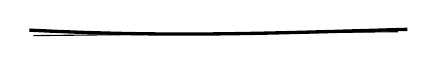
\begin{tikzpicture}\draw[very thick] (0,0) .. controls (1.8,-0.09) and (3.0,-0.04) .. (4.8,0.01);\draw (0.05,-0.07)--(4.68,-0.02);\end{tikzpicture}}

\diagram{\begin{tikzcd}[column sep=small,row sep=small]
A/Q.Q'\longrightarrow A/Q\unsure{\times|+}A/Q' & \text{surjectif }\deleted{\unsure{ssi}} \arrow[d,Leftrightarrow] & \\
& \text{bijectif} \arrow[d,Leftrightarrow] & \\
& Q+Q'=A \arrow[r,Rightarrow] & QQ'=Q\cap Q'
\end{tikzcd}}
